\documentclass[12pt]{report}
\usepackage[utf8]{inputenc}
\usepackage{graphicx}
\usepackage[spanish]{babel}
\usepackage{verbatim} 
\usepackage{amsmath}
\graphicspath{ {img/} }
\setcounter{tocdepth}{3}
\setcounter{secnumdepth}{3}
\usepackage{gensymb}
\usepackage{multicol}

\begin{document}

\begin{titlepage}

\begin{center}
\vspace*{-1in}
\begin{figure}[htb]
\begin{center}
\includegraphics[width=3.5cm]{./img/chapter0/logouv2.jpg}
\end{center}
\end{figure}
\begin{Large}
Universidad Veracruzana
\\
\vspace*{0.15in}
Facultad de Ingeniería de la construcción y el habitat \\
\vspace*{0.6in}
\end{Large}
\begin{large}
TESIS:\\
\end{large}
\vspace*{0.2in}
\begin{Large}
\textbf{Diseño y construcción de un brazo robótico colaborativo para sistemas de manufactura flexible} \\
\end{Large}
\vspace*{0.3in}
\begin{large}
Presenta Ángel Ernesto Trujillo Elizondo, para obtener el grado de Maestría en Ingeniería Aplicada\\
\end{large}
\vspace*{0.3in}
\rule{80mm}{0.1mm}\\
\vspace*{0.1in}
\begin{large}
Asesor: \\
José Alejandro Vasquez Santacruz \\
\end{large}
\end{center}
\end{titlepage}


\tableofcontents
\listoffigures
\listoftables

\chapter*{Agradecimientos} 
\addcontentsline{toc}{chapter}{Agradecimientos}

Agradezco al Consejo Nacional de Ciencia y Tecnología por el apoyo económico recibido durante la realización de este posgrado.

Agradezco profundamente a mi asesor, el Dr. José Alejandro Vásquez Santacruz por su apoyo y paciencia durante la realización de esta investigación.

\chapter*{Resumen}
\addcontentsline{toc}{chapter}{Resumen}

Aquí va un resumen, pero cuando acabe.

\chapter*{Abstract}
\addcontentsline{toc}{chapter}{Abstract}

Here goes an abstract, but i'll do it when I finish.


\chapter{Introducción}

El propósito de esta investigación consiste en desarrollar un brazo robótico colaborativo de coste accesible para que las pequeñas y medianas empresas puedan aumentar la eficiencia y calidad en sus procesos así como librar a sus trabajadores de tareas repetitivas o potencialmente peligrosas. %This was five.

Aún con el crecimiento en la demanda de los robots colaborativos, el precio de éstos no ha sufrido grandes cambios desde su lanzamiento, pues su precio promedio ronda en los \textbf{\$50,000 dólares}, lo cual es prohibitivo para las pequeñas y medianas empresas. % This was four.

Los robots colaborativos, también denominados \textit{cobots}, son aquellos que permiten a los humanos ocupar la misma área de trabajo que éstos y ofrecer la interacción segura entre robot y humano con el fin de realizar una tarea común.  % This was the first.

Los \textit{cobots} ofrecen mucho más flexibilidad en su operación con respecto a los robots industriales tradicionales. Las desventajas consisten en sacrificar la carga útil máxima así como la  eficiencia y el alcance de los robots industriales tradicionales. En resumen, los robots colaborativos son un excelente compromiso entre el trabajo manual y la automatización industrial. \cite{Zaatari2019} % This was second.

El interés en los robots colaborativos ha ido en aumento en la última década, es por esto que los grandes fabricantes de robots como ABB, KUKA o Universal Robots han desarrollado productos para este nicho de mercado. Por su parte, las grandes emprezas de manufactura como Audi, Volkswagen y Nissan han incorporado robots colaborativos en sus lineas de ensamblaje. \cite{Zaatari2019} % And third.

\begin{comment}
Párrafo uno: Introducción sobre los robots colaborativos
Párrafo dos: Ventajas con respecto a robots tradicionales
Párrafo tres: Pertinencia de la investigación en la actualidad
Párrafo cuatro: Propósito de la investigación.
Párrafo cinco: Propósito de la investigación e interés social.
\end{comment}


\section{Objetivos}

El objetivo general de esta investigación consiste en diseñar y construir un brazo robótico colaborativo de seis grados de libertad para sistemas de manufactura flexible.

Los objetivos específicos se mencionan a continuación:

\begin{itemize}
\item Desarrollar el modelo matemático cinemático y dinámico de un brazo robótico de seis grados de libertad.
\item Construir un brazo robótico de coste accesible y fácil fabricación, así como compartir su diseño y componentes con una licencia de código abierto. 
\item Optimizar el modelado de piezas para su correcta manufactura con máquinas de manufactura aditiva.
\item Desarrollar ¿utilizar? una metodología apegada a la ingeniería de sistemas basadas en modelos.
\end{itemize}

\section{Justificación}

El desarrollo de un brazo robótico de seis grados de libertad para sistemas de manufactura flexible que se pretende realizar es relevante en diversos ámbitos del conocimiento. 

Por último, al estar pensado como un desarrollo de código abierto, contribuirá al acervo tecnológico de la humanidad y podrá ser copiado, modificado y mejorado alrededor del mundo. 


\section{Hipótesis}


\chapter{Marco teórico}

\section{Brazos robóticos industriales}

Antes de entrar en el tema principal de este documento, es importante conocer el antecedente o lo que se trata de mejorar, en nuestro caso, es imposible hablar de robots colaborativos sin primero abordar los brazos robóticos industriales.

Un brazo robótico es un manipulador, usualmente programable con funciones similares a las de un brazo humano. Los eslabones de este manipulador estan conectados por articulaciones que permiten el movimiento rotacional o translacional. \cite{ReviewRoboticArm} \cite{Schilling2001}

De acuerdo con \cite{Spong2005}, la mayoría de las aplicaciones en el campo de la robótica se centran en brazos robóticos industriales que operan en fabricas con entornos estructurados, es por esto su gran importancia.

La Federación Internacional de Robótica ha reportado un crecimiento promedio anual a partir del 2013 del 19\% en la demanda de brazos robóticos, siendo la industria automotríz la dominante, seguida por la industria eléctrica y electrónica. \cite{summary2019}


\subsection{Clasificación de los robots}

La clasificación de los brazos robóticos tiene dos grandes ramas, una de estas es por la fuente de su energía y la otra por la geometría de trabajo. 

La fuente de energía puede ser eléctrica o hidráulaca, la mayoría de los manipuladores hoy en día usan servomotores o motores a pasos de corriente continua \cite{Schilling2001}.

Dependiendo de la geometría de trabajo, los brazos robóticos  se dividen en: cartesianos, cilíndricos, esféricos, SCARA o articulados.


\section{Robótica colaborativa}

La robótica colaborativa surge como una rama de la robótica dispuesta a hacer más fácil el trabajo en lineas de producción, así como aliviar problemas en la espalda relacionados con tareas de ensamblado final en posiciones no ergonómicas \cite{cobot2018}\cite{cobotreview}.

Los robots colaborativos han sido desarrollados para trabajar de manera segura al lado de humanos, tomando en consideración la seguridad del operador, la del mismo robot y la correcta realización de la tarea a realizar.  Por esto, están equipados con medidas de seguridad para reconocer el ambiente en el que trabajan, tales como sistemas de evasión de obstáculos y detección de colisiones, implementadas a través de sensores o de mecanismos de compilación pasiva.

\paragraph{Escenarios de colaboración.} Es claro que no todas las aplicaciones donde se implemente un robot colaborativo requieren las mismas consideraciones, es por esto que existe una clasificación de acuerdo al grado de interacción con el operador y la dependencia entre éste y el robot colaborativo. Esos escenarios se mencionan a continuación y se ilustran en la figura \ref{fig:escenarioscolaborativos} \cite{Zaatari2019}.


\begin{itemize}
\itemsep0em
\item \textbf{Independiente.} Un operador y un robot colaborativo trabajan en distintas piezas de trabajo, cada uno con un proceso de manufactura individual. El elemento colaborativo es debido a la co-presencia en la misma área de trabajo.
\item \textbf{Simultanea.} Un operador y un robot colaborativo operan en procesos separados en la misma pieza de trabajo al mismo tiempo. No existe una dependencia de tarea entre ellos, sin embargo, el cobot debe estar conciente y respetar el espacio del operador.
\item \textbf{Secuencial.} Un operador y un cobot relizan un proceso de manufactura secuencial en la misma pieza de trabajo. Existe dependencia de tiempo entre ambos a lo largo del proceso.
\item \textbf{Soporte.} Un operador y un robot trabajan en el mismo proceso de manera interaciva. Existe una dependencia entre las acciones del robot y el operador, es decir, sin uno de ellos, la tarea no podría realizarse.
\end{itemize}

\begin{figure}
    \centering
    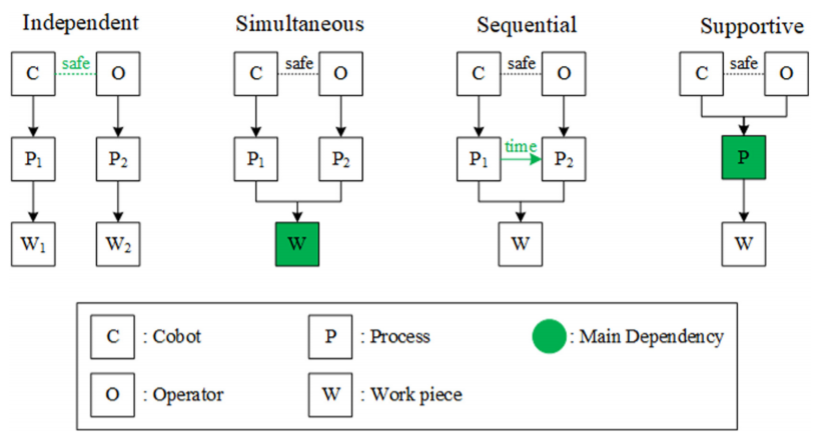
\includegraphics[scale=0.8]{./img/chapter2/escenarioscolaborativos.png}
    \caption{Escenarios colaborativos}
    \label{fig:escenarioscolaborativos}
\end{figure}

Con esto en mente, es fácil deducir que la mayoría de las investigaciones en el área de robótica colaborativa están encaminadas a estudiar o mejorar la detección de colisiones para salvaguardar la integridad de las personas que deberán trabajar junto a los cobots.

Incluso antes de que se acuñara el término cobots, ya había investigaciones encaminadas a la evasión de obstáculos \cite{Khatib1986}, dónde se plantea la solución a través de algoritmos de planeación de ruta.


En la mayoría de los robots colaborativos que existen en el mercado hoy en día se utilizan sensores de fuerza-torque en cada una de las articulaciones, sin embargo, los sensores montados en el robot colaborativo no son la única forma de proveer la seguridad necesaria, en \cite{Teke2018}, se aborda el uso de sensores de visión computacional a través del dispositivo Kinect V2 de Microsoft para modificar la trayectoria y así evadir obstáculos.

En \cite{Lu2005}, se concluye que es posible detectar colisiones utilizando sensores de fuerza-torque únicamente en la base y muñeca de un brazo robótico. Los sensores de fuerza-torque son sumamente caros, por esta razón existen investigaciones como \cite{Phan2018} donde se trabaja en desarrollar nuevos sensores de fuerza-torque con gran velocidad de respuesta y bajo costo.

De igual forma, se han desarrollado estudios sobre como es posible desarrollar robots colaborativos sin la necesidad de sensores de fuerza-torque.

En \cite{Matsumotoa}, se propone un método de detección de colisión basado en la ley de control no-lineal adaptativo, donde se utiliza la diferencia entre el torque obtenido realmente en contra del calculado basado en el modelo dinámico.

Por otra parte, en \cite{Chen2018} también se propone el desarollo de un algoritmo de detección de colisión basado en el modelo dinámico del robot, en este se utiliza la corriente suministrada al motor y la información que proporcionen los sensores de posición para medir discrepancias y detectar colisiones, lo que reduce el costo dedicado a sensores que requiere un robot colaborativo. En esta investigación se tratará de replicar esta metodología para lograr un algoritmo de detección de colisión.

Uno de los ejemplos más populares de robots colaborativos es la línea de robots UR creada por Universal Robots, quién ha vendido más de 39,000 unidades de estos cobots. Una imagen del mismo puede ser apreciada en la figura \ref{fig:ur5}.

\begin{figure}
    \centering
    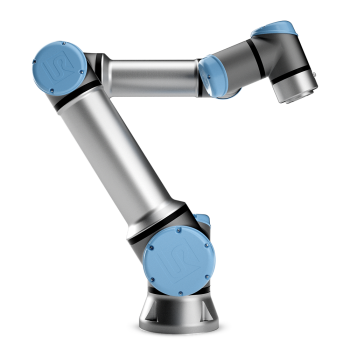
\includegraphics[scale=0.5]{./img/chapter2/ur5.png}
    \caption{Robot colaborativo UR5 de Universal Robots}
    \label{fig:ur5}
\end{figure}

\section{Sistemas de manufactura flexible}
\section{Ingeniería de sistemas basado en modelos}

\chapter{Metodología}

\section{Modelos matemáticos}

De acuerdo con \cite{Dombre2007}, el diseño y control de robots requiere diversos modelos matemáticos, tales como:

\begin{itemize}
\itemsep0em 

\item Cinemática directa e inversa, es decir, encontrar la posición del efector final en términos de las coordenadas de las articulaciones y viceversa.
\item Cinemática de la velocidad, encontrar la velocidad del efector final en términos de la velocidad de las articulaciones y viceversa.
\item Modelo dinámico, el cual establece la relación entre los torques o fuerzas que ejercen los actuadores y las posiciones, velocidades y aceleraciones de las articulaciones.
\end{itemize}

\begin{figure}
    \centering
    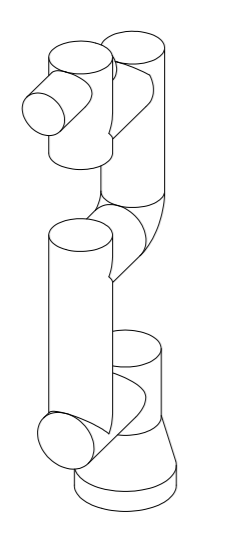
\includegraphics[scale=0.7]{./img/chapter3/robotarmprototype.png}
    \caption{Boceto del brazo robótico propuesto}
    \label{fig:roboticarmprototype}
\end{figure}

En este capítulo se desarrollarán los modelos matemáticos necesarios para simular y diseñar el brazo robótico, así como predecir el comportamiento del mismo.

Para realizar estos modelos, es importante contar con los parámetros físicos y geométricos del robot, los cuales aún no están completamente definidos, por lo que, para una primera aproximación, se utilizarán valores experimentales. Éstos se mencionan en la tabla \ref{table:parametrosbrazorobotico}.

Otros parámetros necesarios para el desarrollo del modelo matemático del brazo robótico son el alcance total del brazo, el cual deberá ser de mínimo 500 mm, la velocidad, la cuál deberá estar en un rango entre 5 RPM y 30 RPM, y por último, la carga útil, la cuál deberá ser de 2 kg.

\begin{table}
\centering
\caption{Parámetros del brazo robótico}
 \label{table:parametrosbrazorobotico}
\begin{tabular}{l|l|l|l|l|l|l|}
\textbf{Eslabones}                       &  1   &  2   &  3   &  4   &  5   &  6    \\ 
\hline
Longitud           & 0.152       & 0.104       & 0.244       & 0.104       & 0.213       & 0.104        \\
Masa               & 0           & 2           & 1           & 0.8         & 0.8         & 0.2          \\
Centro de gravedad & {[}0, 0, 0] & {[}0, 0, 0] & {[}0, 0, 0] & {[}0, 0, 0] & {[}0, 0, 0] & {[}0, 0, 0]  \\
Matriz de inercia      & {[}0, 0, 0] & {[}0, 0, 0] & {[}0, 0, 0] & {[}0, 0, 0] & {[}0, 0, 0] & {[}0, 0, 0]  \\
Fricción en eslabón    & 0.00148     & 0.00817     & 0.00138     & 7.12e-05    & 8.26e-05    & 3.67e-05     \\
Fricción de Coulomb    & 0.395       & 0.126       & 0.132       & 0.0113      & 0.00926     & 0.00396      \\
Inercia del motor      & 0.002       & 0.002       & 0.002       & 3.3e-05     & 3.3e-05     & 3.3e-05     
\end{tabular}
\end{table}

En la figura \ref{fig:roboticarmprototype} podemos ver un boceto del brazo robótico que se planea implementar.

Con estos datos definidos, es posible empezar la realización de los modelos matemáticos.

\subsection{Cinemática directa e inversa.}

En esta sección se desarrollará el primer modelo matemático del brazo robótico, la cinemática directa e inversa, la cual se trata de encontrar la posición final del brazo dependiendo de las coordenadas $\theta$ de sus articulaciones o, para el caso de la cinemática inversa, calcular las coordenadas $\theta$ necesarias para llegar a una posición $(x,y,z)$ dada.

\subsubsection{Cinemática directa} 
Como ya se mencionó anteriormente, la cinemática directa de un brazo robótico se refiere al cálculo de la posición y orientación del marco de referencia del efector final a partir de las coordenadas $\theta$ de sus articulaciones. \cite{University2017}

Un ejemplo de esto lo podemos encontrar en la figura \ref{fig:forwardkinematic2}, donde se analiza la cinemática directa de un brazo robótico de tres grados de libertad. En este ejemplo podemos apreciar que la longitud de los eslabones se representan como $L_1, L_2, L_3$ respectivamente y se ha escogido un marco de referencia fijo denominado \{0\}, mientras que el marco de referencia del efector final es \{4\}. \cite{University2017}

Entonces, para conocer la posición final es necesaria la siguente ecuación:
\begin{equation}
\label{eq:cinematicadirecta1}
x = L_1 \cos(\theta_1)+L_2 \cos(\theta_1 + \theta_2)+ L_3 \cos(\theta_1 + \theta_2 + \theta_3)
\end{equation}
\begin{equation}
\label{eq:cinematicadirecta2}
y = L_1 \sin(\theta_1)+L_2 \sin(\theta_1 + \theta_2)+ L_3 \sin(\theta_1 + \theta_2 + \theta_3)
\end{equation}
\begin{equation}
\label{eq:cinematicadirecta3}
\phi = \theta_1 + \theta_2 + \theta_3
\end{equation}

Las ecuaciones \ref{eq:cinematicadirecta1}, \ref{eq:cinematicadirecta2} y \ref{eq:cinematicadirecta3} se les conoce como \textbf{ecuación de cinemática directa} y aunque es válida, se vuelve rápidamente compleja para un brazo robótico de seis grados de libertad, por esta razón, el enfoque sistemático de resolución es utilizar matrices de transformación homogenea y la convención de Denavit-Hartenberg.

\begin{figure}
    \centering
    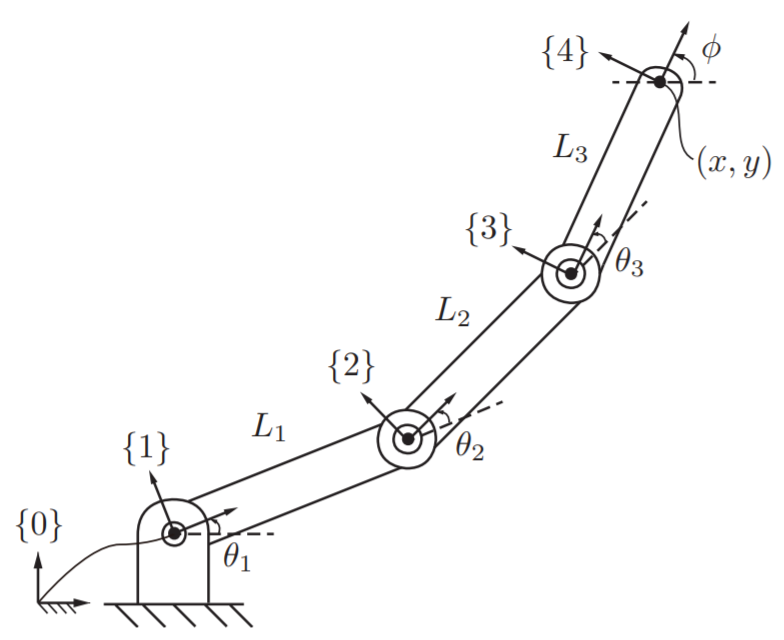
\includegraphics[scale=0.6]{./img/chapter3/forwardkinematic.png}
    \caption{Cinemática directa de un brazo robótico de 3 grados de libertad \cite{University2017}}
    \label{fig:forwardkinematic2}
\end{figure}

\paragraph{Matriz de transformación homogénea.}

Una matriz de transformación homogenea no es nada más que la representación matricial de un movimiento rígido \cite{Spong2005}, así, la posición y orientación del efector final puede ser fácilmente calculada utilizando multiplicación de matrices.

La forma más general de una matriz de transformación homogenea puede ser escrita de la siguiente manera:

\begin{equation}
T^0_1 =
\begin{bmatrix}
n_x & s_x & a_x & d_x\\
n_y & s_y & a_y & d_y\\
n_z & s_z & a_z & d_z\\
0 & 0 & 0 & 1
\end{bmatrix} = 
\begin{bmatrix}
n & s & a & d\\
0 & 0 & 0 & 1
\end{bmatrix}
\end{equation}

En dónde $n$ es un vector representando la dirección $x_1$ en el sistema $o_0 x_0 y_0 z_0$, de manera similar, $s$ representa la dirección de $y_1$ y $a$ representa la direción de $z_1$. Por su parte, $d$ es un vector representando la posición desde el origen $o_0$ hasta el origen $o_1$ en el marco de referencia $o_0 x_0 y_0 z_0$.


Según \cite{University2017}, existen tres usos principales para una matriz de transformación homogénea:

\begin{enumerate}
\itemsep0em
  \item Para representar la configuración (posición y orientación) de un cuerpo rígido.
  \item Para cambiar el marco de referencia en el cuál está representado un vector u otro marco de referencia.
  \item Para desplazar un vector o un marco de referencia.
\end{enumerate}

Para el caso que nos ocupa, necesitamos la matriz de transformación homogénea desde la base fija del robot hasta su efector final, descrita con la ecuación siguiente:
\begin{equation}
\label{eq:homogeneustransformationmatrix}
\begin{split}
{}_{0}^{7}T = \mathscr{T}_z(a_1)\oplus\mathscr{R}_z(\theta_1)\oplus\mathscr{T}_x(b_1)\oplus\mathscr{R}_x(\theta_2)\oplus\mathscr{T}_z(c_1)\oplus\mathscr{R}_x(\theta_3) \\ \oplus\mathscr{T}_z(d_1)\oplus\mathscr{T}_x(d_2)\oplus\mathscr{R}_x(\theta_4)\oplus\mathscr{T}_x(e_1)\oplus\mathscr{R}_z(\theta_5)\oplus\mathscr{T}_z(f_1)\oplus\mathscr{R}_x(\theta_6)
\end{split}
\end{equation}

Dónde $a_1, b_1, c_1, d_1, d_2, e_1$ y $f_1$ son las longitudes de los eslabones del brazo robótico. 

\begin{figure}
    \centering
    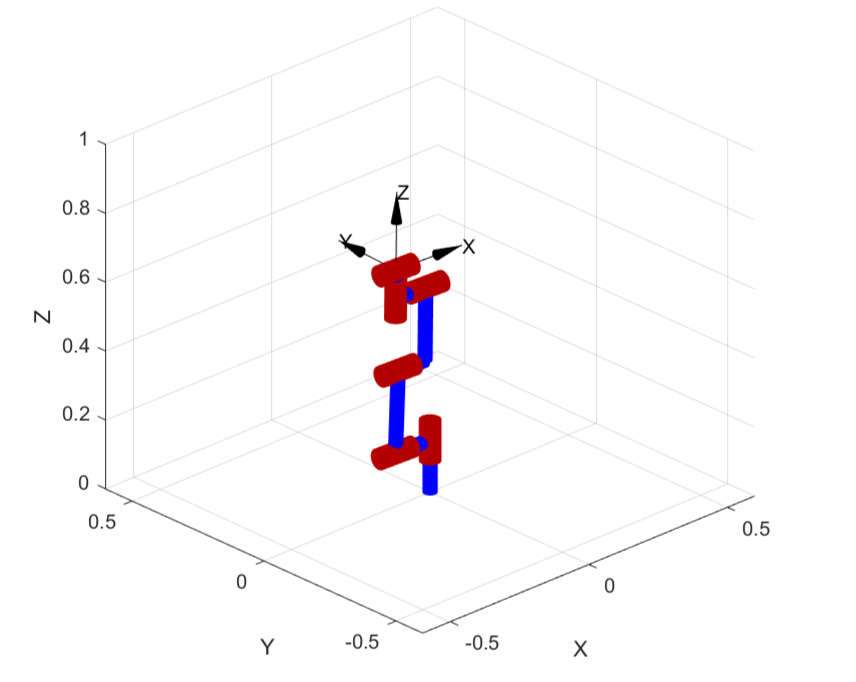
\includegraphics[scale=0.6]{./img/chapter3/KinematicDiagramML.png}
    \caption{Cadena cinemática}
    \label{fig:kinematicchain}
\end{figure}


En la imagen \ref{fig:kinematicchain} podemos observar la cadena cinemática de nuestro brazo robótico, fue creada con un algoritmo en MATLAB con ayuda de la herramienta Robotic Toolbox \cite{Corke2017}, dicho código puede consultarse en el Anexo 1.


\paragraph{Convención de Denavit-Hartenberg.} En muchas aplicaciones, es necesario representar los parámetros cinemáticos de forma simplificada con ayuda de la notación Denavit-Hartenberg, con esta convención se simplifa considerablemente el análisis.

Con esta notación podemos hacer uso de algoritmos de solución para encontrar los valores dinámicos, planeación de trayectorias y simulaciones, entre otros valores.

En \cite{Corke2007}, se propone un acercamiento sencillo y sistemático para convertir una matriz de transformación homogenea como la de la ecuación \ref{eq:homogeneustransformationmatrix} en los parámetros de Denavit-Hartenberg. 

Al realizar dicho proceso se llegó a los resultados que se muestran en la tabla \ref{table:denavithartenberg}.

\begin{table}
\centering
\caption{Parámetros Denavit Hartenberg}
 \label{table:denavithartenberg}
\begin{tabular}{l|l|l|l|l|}
               & $\theta$ [rad] & d [m]    & a [m]   & $\alpha$ [rad]                        \\ 
\hline
Articulación 1 & $\theta_1$              & 0.152    & 0       & $\frac{\pi}{2}$   \\
Articulación 2 & $\theta_2$              & 0        & -0.244       & 0 \\
Articulación 3 & $\theta_3$                  & 0 & -0.213       & 0                                                  \\
Articulación 4 & $\theta_4$              & -0.012        & 0 & $-\frac{\pi}{2}$   \\
Articulación 5 & $\theta_5$                        & 0.085        & 0 & $\frac{\pi}{2}$  \\
Articulación 6 & $\theta_6$                           & 0        & 0  & $-\frac{\pi}{2}$                                                 
\end{tabular}
\end{table}

Con esto, tenemos una vista simplificada de nuestro brazo robótico, que describe su cinemática directa usando únicamente cuatro parámetros por articulación. El algoritmo desarrollado puede consultarse en el Anexo 2.	

\subsubsection{Cinemática inversa}

Una vez terminada la cinemática directa, toca al turno de abordar la cinemática inversa. Hasta este punto podemos calcular la posición del efector final utilizando las variables de las articulaciones, ahora, procederemos a encontrar las variables de las articulaciones dada una posición y orientación del efector final.

Para nuestro caso, un brazo robótico de seis grados de libertad, la solución tiene doce ecuaciones con seis incognitas, sin embargo, nueve ecuaciones se derivan de la matriz de rotación dentro de la matriz de transformación homogenea ${}_{0}^{6}T$, esto deja unicamente tres ecuaciones independientes, agregando las tres ecuaciones del vector de posición dentro de la matriz de transformación homogenea ${}_{0}^{6}T$ nos da como resultado seis ecuaciones con seis incógnitas.	

Estas ecuaciones son no-lineales y transendentales, lo cual hace más dificil encontrar una solución y como cualquier conjunto de ecuaciones no-lineales, puede existir una sola solución o múltiples soluciones. \cite{Craig2013}

Para resolver el problema de encontrar la cinemática inversa existen dos métodos posibles: \textit{la solución de forma cerrada} y la solución numérica. 

El concenso de la mayoría de los autores, tales como \cite{Spong2005} y \cite{Craig2013} es que se prefiere encontrar la solución de forma cerrada por dos razones principales, la velocidad de solución y la forma en la que se encuentra una solución, es decir, como la cinemática inversa puede tener muchas soluciones se pueden desarrollar reglas para favorecer un tipo de solución con respecto de otra.

Exiten algunos artículos como \cite{Chen2017} en el cuál se ejemplifica la manera de resolver la cinemática inversa de un robot manipulador de seis grados de libertad de forma analítica.

Queda claro que resolver la cinemática inversa no es tarea sencilla, por esta razón y de manera parecida a como se manejó en la sección anterior, se utilizará la librería Robotic Toolbox, la cual incluye un método establecido para calcular la cinemática inversa dada una matriz de transformación homogénea. El algoritmo desarrollado puede consultarse en el Anexo 3.

Así mismo, es importante notar que esta solución se utilizará únicamente en la etapa de desarrollo del brazo robótico y se tendrá que implementar un algoritmo de solución de cinemática inversa en el control final del robot.

\subsection{Cinemática de la velocidad}

Soon.

\subsection{Modelo dinámico}

Hasta ahora, se ha descrito el movimiento del robot sin consideración de las fuerzas y los torques necesarios para producir dicho movimiento, ahora toca el turno de analizarlas.

Como se comentó al principio del capítulo, es necesario establecer una relación entre las posiciones, velocidades y aceleraciones deseadas y el torque o fuerzas que se debe ejercer en los actuadores, esto nos permitirá controlar el brazo robótico así como conocer los parámetros necesarios que los actuadores deben cumplir para satisfacer los requerimientos de velocidad y carga útil.

Para lograrlo, existen dos fomulaciones que se pueden seguir, la formulación Euler-Lagrange o la formulación Newton-Euler. Ambos métodos llegarían a la misma respuesta, sin embargo el camino será diferente.

En la formulación Euler-Lagrange se trata al robot como un todo y se realiza el análisis utilizando la formulación Lagraniana (la diferencia entre energía cinética y energía potencial), por su parte, la formulación Newton-Euler divide el manipulador en cada uno de sus eslabones y describe las escuaciones que definen su movimiento lineal y angular. \cite{Spong2005}

En esta parte de la investigación y como parte de los modelos matemáticos necesarios para seguir diseñando el robot, se utilizará la \textit{formulación Newton-Euler} para obtener los torques y fuerzas necesarias. 

\subsubsection{Formulación Newton-Euler}

Para encontrar los torques a los que deben estar sometidos las articulaciones del brazo robótico se utilizará la herramienta que se ha utilizado a lo largo de este capítulo, con ella, se desarrolla un algoritmo en MATLAB donde se incluiyen los parámetros necesarios para el modelo dinámico tales como masa, centro de gravedad, momento de inercia, fricción viscosa, fricción de Coulomb, inercia del motor y relación de engranes. 

La lista de parámetros para cada articulación y eslabón fue descrita anteriormente en el cuadro \ref{table:parametrosbrazorobotico}.

Cabe destacar que algunos de los parámetros dinámicos son una aproximación optimista, esto debido a no tener aún un diseño final ni todos los componentes seleccionados, sin embargo, es funcional para una primera iteración del torque necesario para continuar con la selección de componentes.

Con los datos del cuadro \ref{table:parametrosbrazorobotico} se selecciona los torques máximos en el escenario más demandante, esto es en una trayectoria en la cuál cada una de las articulaciones se somete a una mayor fuerza.

Con todos los datos correctamente particularizados, obtenemos una lista con todos los valores máximos, se puede apreciar en el cuadro \ref{table:maxtorque}. 

\begin{table}
\centering
\caption{Parámetros del brazo robótico}
\label{table:maxtorque}
\begin{tabular}{l|l|l|l|l|l|l|}
\textbf{Articulaciones}              &  1 & 2 & 3 &  4 &  5 &  6  \\ 
\hline
Torque máximo (N) & 0.2            & 25.35          & 11.94~         & 2.33           & 0.2            & 0.2            
\end{tabular}
\end{table}

El algoritmo realizado está disponible para consulta en el Anexo 4. Así como el repositorio de esta tésis.
       
\section{Componentes eléctricos y electrónicos}

Conforme al análisis realizado en el capítulo anterior es posible empezar la selección de componentes, se empezará por la selección de motores.

Conforme a lo expuesto en el capítulo \ref{chap:Marcoteorico}, se optó por utilizar motores de corriente continua sin escobillas, conocidos también por sus siglas en inglés BLDC.

De acuerdo con los datos proporcionados por la tabla \ref{table:maxtorque}, la articulación con un torque más demandante es la articulación dos, conocida como el hombro del robot, esta necesita un torque total de 25 N para levantar una carga útil de 2 Kg. Siendo esta la parte más desafiante del brazo robótico, se empezará por el desarrollo de ésta.

Es prácticamente imposible encontrar un motor con ese torque, por lo que será necesario utilizar un sistema de engranes reductores, por ahora, se seleccionará un motor con un torque de salida de entre 1.5 y 2 N para incremenentar el torque de salida a través de engranajes.

Se seleccionó un motor de la marca Turnigy, en particular el modelo Aerodrive SK3 - 6374-149KV, pues según datos experimentales realizados en \cite{odrivedoc} tiene un torque máximo de 3.77 N. Es posible apreciar una imagen de este motor en la figura \ref{fig:sk36374}.

\begin{figure}
    \centering
    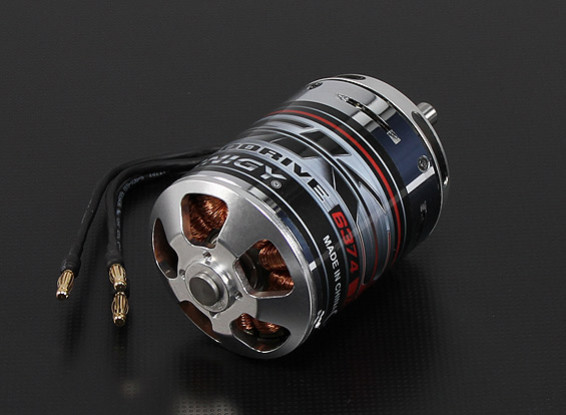
\includegraphics[scale=0.6]{./img/chapter3/sk36374.jpg}
    \caption{Motor a utilizar en la articulación dos.}
    \label{fig:sk36374}
\end{figure}


\section{Componentes mecánicos}

Una vez determinado los componentes electrónicos necesarios para el correcto funcionamiento del brazo robótico es necesario determinar los componentes mecánicos.

\subsection{Actuadores}

Una de las partes mecánicas más importantes es el actuador, es decir, el mecanismo que proporcionará la fuerza necesaria para mover las articulaciones del robot.

Para la correcta selección o desarrollo del actuador necesitamos dos parámetros que vimos en los capítulos anteriores, el primero es el torque necesario para realizar los desplazamientos del robot a la velocidades y aceleraciones requeridas y el segundo es la velocidad nominal del motor a utilizar.

Por norma general, los motores eléctricos y, para nuestro caso, los motores eléctricos sin escobillas, funcionan a velocidades altas y un torque relativamente pequeño, para esto es necesario utilizar reductores de velocidad, los cuales cumplen dos objetivos primordiales: reducir la velocidad en eje de salida y aumentar el torque en el mismo.

El siguiente paso es escoger un reductor de velocidad que cumpla con los requerimientos específicos de nuestro brazo robótico, los cuales son:

\begin{itemize}
\itemsep0em
\item Alta relación de transmisión, mayor a 10:1.
\item Precisión, necesaria para realizar los movimientos deseados sin demasiado juego. 
\item Efectividad de transmisión, necesaria para no perder demasiada energía.
\end{itemize}

Estos son algunos de los más importantes, existen otros factores a considerar como el tamaño final del reductor y la facilidad de manufactura.

Para el desarrollo de este brazo robótico se han considerado tres diferentes tipos de reductores de velocidad, cada uno con ventajas y desventajas que se mencionaron en la sección \ref{sec:actuadores}. Se decidió optar por un reductor cicloidal, esto debido a su gran relación de transmisión y un juego teórico nulo.  

Para el diseño de este actuador se consultaron diferentes fuentes como \cite{Lei2012} \cite{Nachimowicz2016}, y se utilizó la siguiente formula para el diseño paramétrico en SolidWorks.
\begin{equation}
B_x = r  \cdot \cos(\varphi) - q \cdot \cos(\varphi + \Psi) - e \cdot \cos(N\varphi)
\end{equation}
\begin{equation}
B_y = r  \cdot \sin(\varphi) + q \cdot \sin(\varphi + \Psi) + e \cdot \sin(N\varphi)
\end{equation}

Dónde:

$r$ es la distancia entre el engrane central y los rollers en milímetros.
$q$ es el radio del roller en milímetros.
$e$ es el valor de la excentricidad en milímetros.
$N$ es el número de rollers.
$\Psi$ es el angulo entre $B$ y el punto central del sistema coordenado.

Para calcular $\Psi$ se utiliza la siguiente fórmula:

\begin{equation}
\Psi = \tanh \left[ \frac{\sin((1-N)\varphi)}{\frac{r}{eN}-\cos((1-N)\varphi} \right]
\end{equation}
Desde:
$$
0 \leq \theta \leq 360
$$

Los datos de diseño del engrane cicloidal los podemos apreciar en la tabla \ref{table:valorescicloidal}

\begin{table}
\centering
\caption{Valores de diseño del engrane cicloidal.}
\label{table:valorescicloidal}
\begin{tabular}{l|l|l|}
\textbf{Descripción} & \textbf{Símbolo} & \textbf{Valor}  \\ 
\hline
Diámetro del engrane & D                & 80 mm.          \\
Diámetro del roller  & d                & 5 mm.           \\
Número de rollers    & N                & 25              \\
Excentricidad        & e                & 1 mm.          
\end{tabular}
\end{table}

  
\chapter{Modelo matemático}

\section{Modelo cinemático}
\subsection{Matriz de transformación homogénea}



\begin{figure}
    \centering
    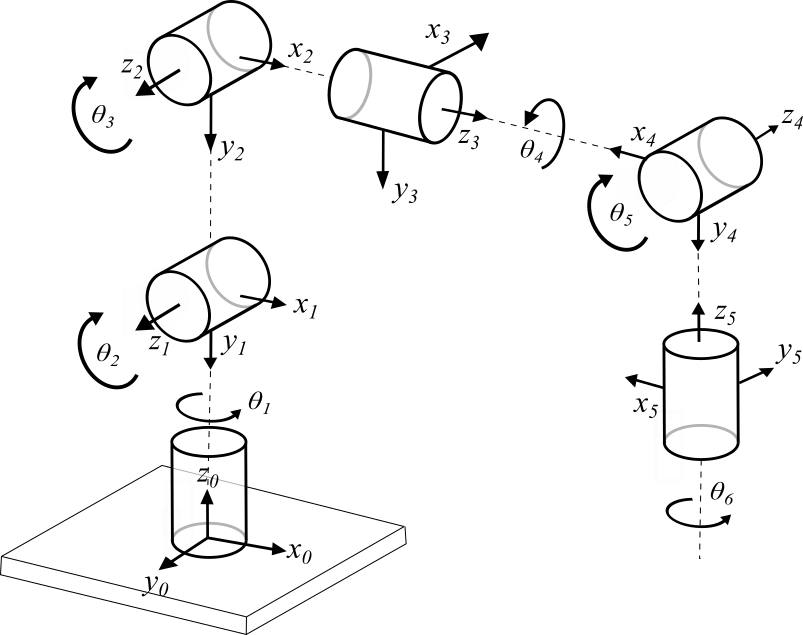
\includegraphics[width=\textwidth]{./img/chapter4/kinematicchainv4.png}
    \caption{Cadena cinemática ¿free body diagram?}
    \label{fig:kinematicchain}
\end{figure}

\[
{}_{0}^{1}T = 
\begin{bmatrix}
    1 & 0 & 0 & 120  \\
    0 & \cos{\theta} & -\sin{\theta} & 0 \\
    0 & \sin{\theta} & \cos{\theta} & 0 \\
    0 & 0 & 0 & 1
\end{bmatrix}
\]


\bibliography{references}
\addcontentsline{toc}{chapter}{Bibliografía}
\bibliographystyle{ieeetr} 

\chapter*{Anexos}
\addcontentsline{toc}{chapter}{Anexos}
\section*{Anexo 1. Función de creación del brazo robótico}
\addcontentsline{toc}{section}{Anexo 1. Función de creación del brazo robótico}

\lstinputlisting[style=Matlab-editor]{./MATLAB/myroboticarm.m}

\section*{Anexo 2. Cinemática directa}
\addcontentsline{toc}{section}{Anexo 2. Cinemática directa}

\lstinputlisting[style=Matlab-editor]{./MATLAB/Anexo2.m}

\section*{Anexo 3. Cinemática inversa}
\addcontentsline{toc}{section}{Anexo 2. Cinemática directa}

\lstinputlisting[style=Matlab-editor]{./MATLAB/Anexo3.m}

\begin{comment}
Dudas:
Capítulo 1.
* Al inicio del marco teórico de la tesis de Jacobo veo que describe los acontecimientos importantes hechos en el área de los robots bípedos y asistenciales, (lo que entiendo como estado del arte, marco teórico), pero hacia el final empieza a explicar conceptos básicos de robótica, algoritmos genéticos y demás.
Capítulo 4.
* Está bien mi cadena cinemática en comparación con el robot UR3?
* Necesito 	un frame para el end-efector?
* El punto de desplazamiento en la matriz de t.h. no debe variar aún con la rotación?
* Tengo dudas en la matriz de transformación homogenea, este video me confunde: https://www.youtube.com/watch?v=tAu8-gkxAcE . Ver la imagen en la carpeta auxiliar.
* Desarrollar la parte dinámica con Lagrange o Newton-Euler


Roadmap:
*Dibujar el brazo robótico
*Realizar el análisis dinámico para calcular torque.

\end{comment}



\end{document}